\section{Marco teórico}
\subsection{Sitios de CQA}
\begin{frame}[allowframebreaks]
	\frametitle{Sitios de CQA}
	Lorem ipsum dolor sit amet, consectetur adipisicing elit, sed do eiusmod tempor incididunt ut labore et dolore magna aliqua.
\end{frame}

\subsection{Sistemas de recomendación}
\begin{frame}[allowframebreaks]
	\frametitle{Sistemas de recomendación}
	Como se mencionó anteriormente, un RS es un conjunto de herramientas de software que sugiere ítems a un usuario, quien posiblemente utilizará algunos de ellos.
\end{frame}

\subsection{Sistemas de recomendación}
\begin{frame}
	\frametitle{Técnicas de Recomendación}
	Los RS basan sus estrategias de recomendaciones en 6 técnicas básicas (Ricci et al., 2011):
	\begin{itemize} [<+>]
		\item Basados en contenido.
		\item FIltrado Colaborativo.
		\item Demográficos.
		\item Basados en conocimiento.
		\item Basados en comunidades (sociales).
		\item Sistemas Híbridos.
	\end{itemize}
\end{frame}

\subsection{Big Data y Arquitecturas}
\begin{frame}[allowframebreaks]
	\frametitle{Sistemas de recomendación}
	Lorem ipsum dolor sit amet, consectetur adipisicing elit, sed do eiusmod tempor incididunt ut labore et dolore magna aliqua.
\end{frame}

\subsection{Medidas de distancia de texto}
\begin{frame}[allowframebreaks]
	\frametitle{Conceptos básicos}
	Lorem ipsum dolor sit amet, consectetur adipisicing elit, sed do eiusmod tempor incididunt ut labore et dolore magna aliqua.
\end{frame}

\begin{frame}[allowframebreaks]
	\frametitle{Medidas utilizadas en este trabajo}
	Lorem ipsum dolor sit amet, consectetur adipisicing elit, sed do eiusmod tempor incididunt ut labore et dolore magna aliqua.
\end{frame}

\subsection{Ensamble de Clustering}
\begin{frame}[allowframebreaks]
	\frametitle{Clustering}
	Lorem ipsum dolor sit amet, consectetur adipisicing elit, sed do eiusmod tempor incididunt ut labore et dolore magna aliqua.
\end{frame}

\begin{frame}
	\frametitle{FastText}
	\begin{itemize}
		\scriptsize
		\item Libreria open-source desarrollada por Facebook.
		\item Basado en Skip-gram pero utilizando un modelo sub-palabra.
		\item Cada palabra es representada como una bolsa de \textit{n-gramas}.
		\item Mayor precisión en diferentes medidas de rendimiento.
	\end{itemize}
\end{frame}

\begin{frame}
	\frametitle{Semantic Distance}
	\begin{itemize}
		\scriptsize
		\item La distancia semántica usada en este trabajo está basada en \textit{redes semánticas} y \textit{estadísticas de corpus} (Li et al., 2006).
		\item Enfocado en textos de distancia corta.
		\item Tiene en cuenta la \textit{información semántica} y la \textit{información del orden} de las palabras implicadas en las frases involucradas.
	\end{itemize}

	\begin{figure}
		\centering
		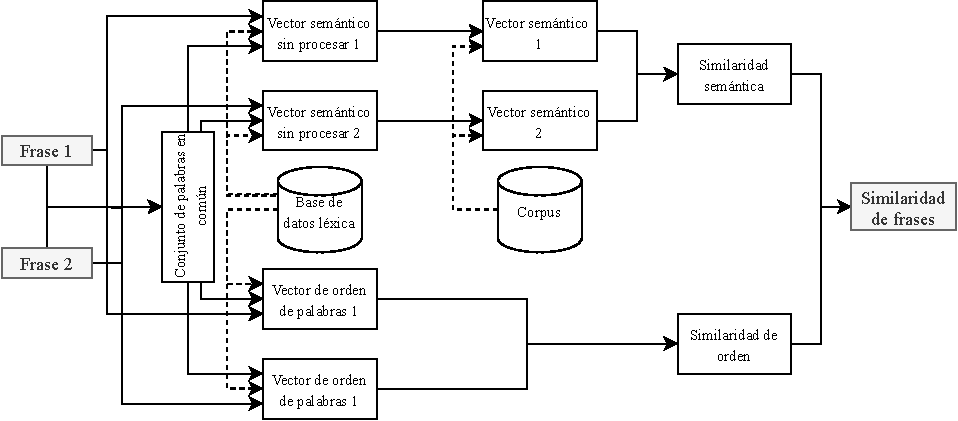
\includegraphics[width=0.7\linewidth]{../7_marco_teorico/imagenes/similaridad_sematinca_metodo}
		\label{fig:similaridadsematincametodo}
	\end{figure}
\end{frame}

\begin{frame}
	\frametitle{Similaridad semántica entre palabras}
	\begin{figure}
		\centering
		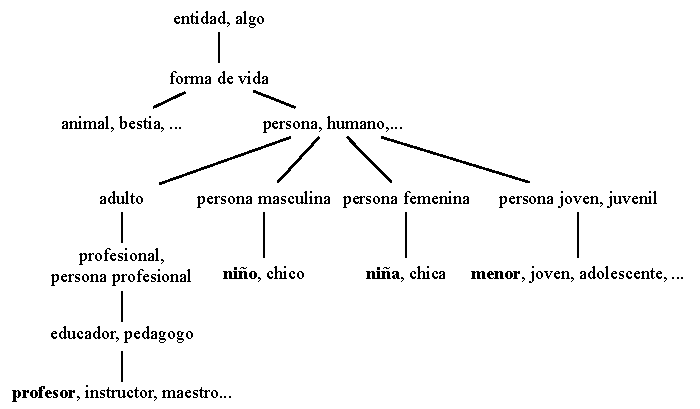
\includegraphics[width=0.7\linewidth]{../7_marco_teorico/imagenes/taxonomia_semantica}
		\label{fig:taxonomiasemantica}
	\end{figure}
\end{frame}

\begin{frame}
	\frametitle{Similaridad semántica entre frases}
	Este método semántico usa únicamente vectores semánticos formados por las frases en comparación. El valor de una entrada del vector semántico es calculado de la siguiente forma:
	\begin{itemize}
		\item \textbf{Caso 1}. Si \(w_i\) aparece en la frase, \(s_i\) es 1.
		\item \textbf{Caso 2}. Si \(w_i\) no está contenida en \(T_1\), se calcula una similaridad semántica entre \(w_1\) y cada palabra en \(T_1\) utilizando el método de la sección anterior.
	\end{itemize}


	Se ponderan cada una de las palabras basadas en su contenido de información:
	\[s_i = \check{s} \cdot I(w_i) \cdot I(\widetilde{w}_i),\]

	La similaridad semántica entre dos frases es definida como el coeficiente del coseno entre los dos vectores:
	\[S_s = \frac{s_1. s_2}{||s_1||.||s_2||}.\]
\end{frame}

\begin{frame}
	\frametitle{Similaridad de orden entre frases}

	Consideremos dos frases \(T_1\) y \(T_2\), por ejemplo:
	\begin{itemize}
		\item \textbf{T1}: A quick brown dog jumps over the lazy fox.
		\item \textbf{T2}. A quick brown fox jumps over the lazy dog.
	\end{itemize}

	\[r_1 = \left \{\;1\;2\;3\;4\;5\;6\;7\;8\;9\;\right \},\]
	\[r_2 = \left \{\;1\;2\;3\;9\;5\;6\;7\;8\;4\;\right \}.\]

	Se propone entonces una medida de similaridad de orden entre frases de la siguiente manera:
	\[S_r = 1 - \frac{\left \| r_1 - r_2 \right \|}{\left \| r_1 + r_2 \right \|}.\]
\end{frame}

\begin{frame}
	\frametitle{Similaridad total entre frases}
	Similaridad total:

	\bigskip
	\[S(T_1, T_2)=\delta S_s + (1 - \delta)S_r,\]
	\[S(T_1, T_2)=\delta \frac{s_1.s_2}{\left \| s_1 \right \|\left \| s_2 \right \|} + (1 - \delta)\frac{\left \|r_1-r_2 \right \|}{\left \| r_1+r_2 \right \|},\]

	\bigskip
	donde \(0 \leq \delta \leq 1\) decide la contribución relativa de cada una de las medidas de similaridad.
\end{frame}

\subsection{Ensamble de Clustering}
\begin{frame}
	\frametitle{Clustering}
	\centering
	El Clustering o \textit{análisis cluster} tiene por objetivo agrupar elementos en grupos homogéneos en función de las similitudes o similaridades entre ellos.
\end{frame}

\begin{frame}
	\frametitle{Ensamble de Clustering}
	\centering
	El \textit{Ensamble de Clustering} es un método para extraer clusters consistentes dadas particiones variadas de entrada.

 	\bigskip

	\begin{itemize}
		\item Combina resultados de distintos algoritmos de Clustering con distintas formas de cluster.
		\item Aprovecha la variabilidad agregada para encontrar una estructura \textit{inter-patrón}.
		\item Identificación de clusters subyacentes con formas, tamaños y densidades arbitrarias.
	\end{itemize}
\end{frame}

\begin{frame}
	\frametitle{Combinación de Evidencias}
	Combinar los resultados de múltiples ejecuciones de clustering dentro de una misma partición de datos viendo cada uno de esos resultados como una evidencia independiente de la organización de los mismos.

	\bigskip

	Tomado las co-ocurrencia de pares de patrones en el mismo cluster, las \(N\) particiones de datos para \(n\) patrones, son mapeadas en una \textit{matriz de co-asociación} \(n \times n\):
	\[C(i,j)=\frac{n_{ij}}{N},\]
	donde \(n_{ij}\) es el número de veces que el par de patrones \((i,j)\) es asignado al mismo cluster entre las \(N\) particiones de datos.
\end{frame}
